Les diagrammes de classes participantes sont représentés dans cette partie. Il y en a un par cas d'utilisation.

\section{Se connecter au bureau distribué}

\noindent\begin{figure}[H]
	\centering
	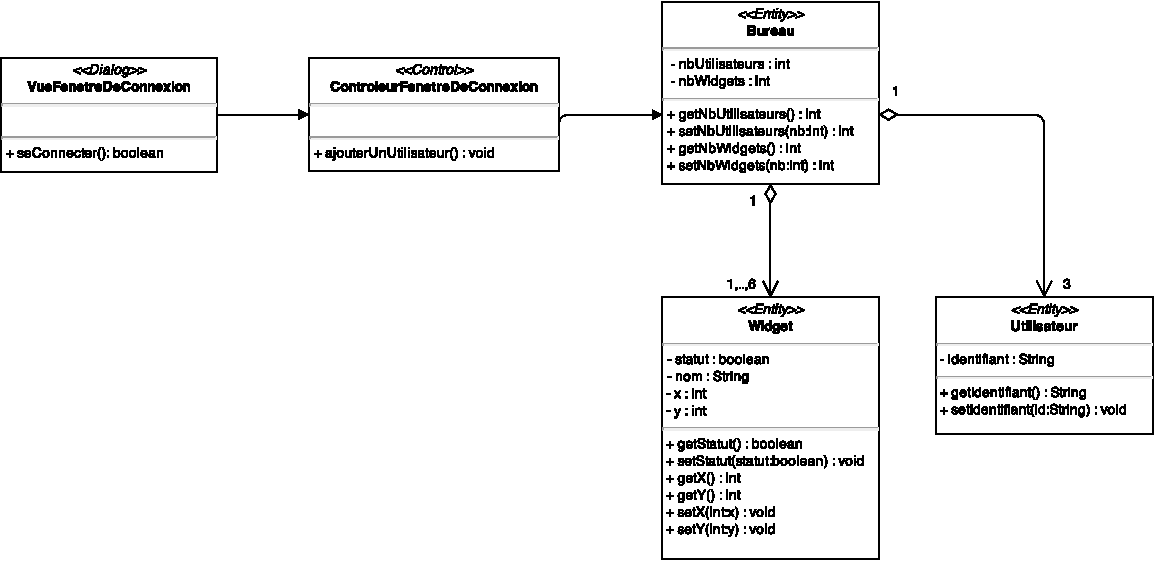
\includegraphics[angle=90]{diagrammes/DCP1.pdf}
	\caption{\color{green}Diagramme de Classes Participantes, cas 1 (modifié)\color{black}}
\end{figure}

\section{Ouvrir une fenêtre}

\begin{figure}[H]
	\centering
	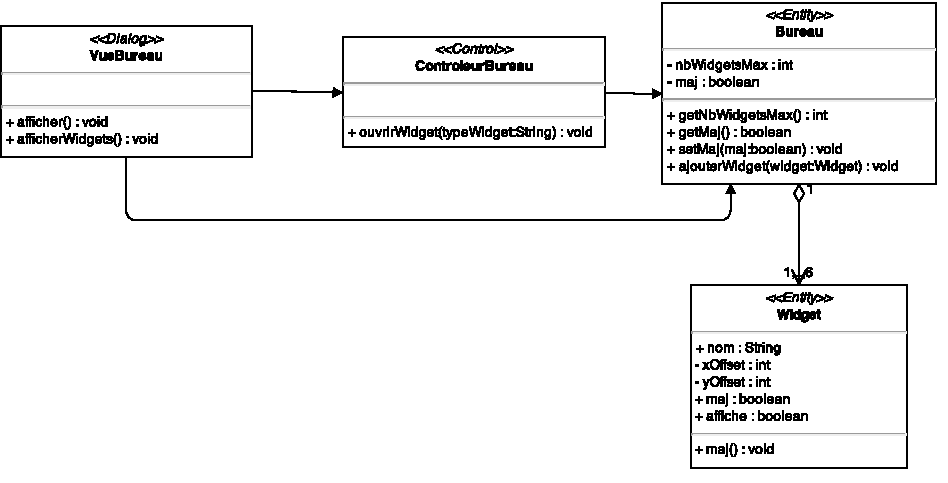
\includegraphics[angle=90]{diagrammes/DCP2.pdf}
	\caption{\color{green}Diagramme de Classes Participantes, cas 2 (modifié)\color{black}}
\end{figure}

\section{\color{red}Saisir une opération (supprimé)}
\noindent\begin{figure}[H]
	\centering
	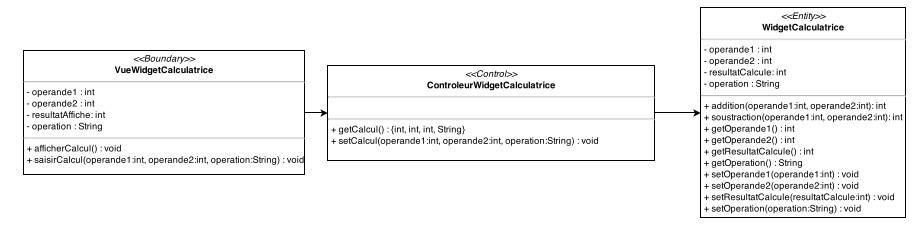
\includegraphics[angle=90,scale=0.9]{diagrammes/DCP4.jpg}
	\caption{\color{red}Diagramme de Classes Participantes, cas 3 (supprimé)\color{black}}
\end{figure}

\section{Regarder des photos}
\begin{figure}[H]
	\centering
	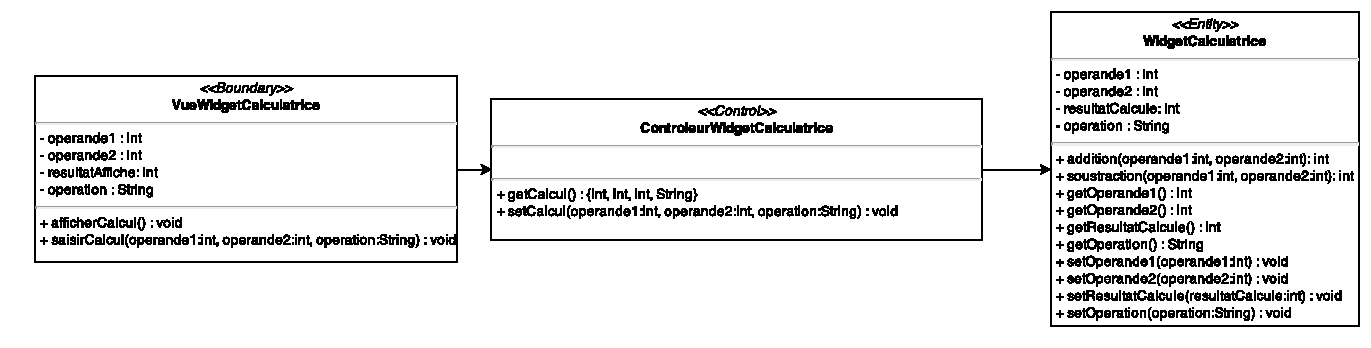
\includegraphics[angle=90]{diagrammes/DCP4.pdf}
	\caption{\color{green}Diagramme de Classes Participantes, cas 3 (modifié)\color{black}}
\end{figure}

\section{Quitter le bureau virtuel}

\begin{figure}[H]
	\centering
	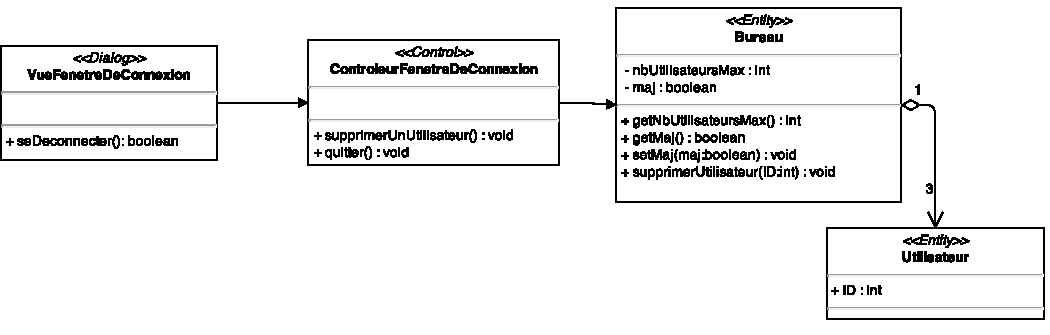
\includegraphics[angle=90]{diagrammes/DCP5.pdf}
	\caption{\color{ForestGreen}Diagramme de Classes Participantes, cas 4 (modifié)\color{black}}
\end{figure}